\documentclass{llncs}
\usepackage{graphicx}
\usepackage{url}
\usepackage{wrapfig}
\usepackage{amssymb}
\usepackage{booktabs}
\usepackage{tabu}
\usepackage{tabularx}
\usepackage[labelfont=bf]{caption}

\newcommand{\clust}[2][k]{#2^{\{#1\}}}

\makeatletter
\newcommand\tablefont{\@setfontsize\tablefont{8.5pt}{8.5}}
\makeatother

% --- TITLE AND AUTHOR INFORMATION
%\title{vote2vec: Dimensionality Reduction Toolkit for Voting Records}
\title{Dimensionality Reduction and Visualisation Tools for Voting Records}
\author{Igor Brigadir\inst{1}, Derek Greene\inst{1}, James P. Cross\inst{2}, P\'{a}draig Cunningham\inst{1}}
\institute{Insight Centre for Data Analytics, University College Dublin, Ireland \\
\email{\{igor.brigadir,derek.greene,padraig.cunningham\}@insight-centre.org} 
\and
School of Politics \& International Relations, University College Dublin, Ireland \\
\email{james.cross@ucd.ie} 
}
% --- END OF PREAMBLE 

% --- START DOCUMENT
\begin{document}
\maketitle

\begin{abstract}
Recorded votes in legislative bodies are an important source of data for political scientists. Voting records can be used to describe parliamentary processes, identify ideological divides between members and reveal the strength of party cohesion. We explore the problem of working with vote data using popular dimensionality reduction techniques and cluster validation methods, as an alternative to more traditional \emph{scaling} techniques. We present results of dimensionality reduction techniques applied to votes from the 6th and 7th European Parliaments, covering activity from 2004 to 2014.
\end{abstract}

\section{Introduction}
As a law making body, votes passed in the European Parliament (EP) can have significant influence on citizens across the European Union. Members of the European Parliament (MEPs) hold power over the majority of EU legislation, as well as decisions on budgets and spending. Analysis of votes is not only of interest to researchers, but many interest groups and industries operating within the EU. To produce insights into legislation and party politics computational approaches are highly dependant on latent variable models---using point estimates to make sense of and test theories using voting records \cite{hix2006dim}, speeches \cite{proksch2010position}, party manifestos \cite{manifesto}, expert surveys \cite{mcelroy2012policy}, and more recently social media data \cite{Barbera2014}.

A common theme in these models is the low dimensional reconstruction of high-dimensional data. Roll call votes, where the vote of each member is recorded are typically represented as a matrix of legislators with \emph{for} and \emph{against} votes, treating abstentions as missing values. Legislators, in this case MEPs, are represented as vectors in $d$ dimensions, where each dimension encodes a vote in some way. \emph{Scaling} methods are then applied to recover point estimates or produce visualisations. Scaling methods essentially perform dimensionality reduction, transforming data in a high-dimensional space to a space with fewer dimensions---an $n$ dimensional space $\mathbb{R}^n$ where $n << d$, typically 2 or 3 dimensions are used to produce interpretable visualisations.

While established methods for inductive scaling of roll call votes exist, there are many other potential alternatives that remain unexplored. We describe four such alternatives in Section \ref{sec:methods}, and formulate a cluster quality-based evaluation approach, highlighting advantages and drawbacks of each method. We make the data for 6th and 7th EU parliaments and Python code to reproduce the approaches on different sets of voting records are made available online\footnote{\url{https://github.com/igorbrigadir/vote2vec}}, so that political science researchers can explore these alternative approaches when analysing vote data.

\section{Related Work}
\label{sec:relatedwork}

The NOMINATE \cite{poole2000congress} family of multidimensional scaling approaches are the most widely adopted methods for estimating ideal points from roll call data, and have been applied to European Parliament roll call vote data in \cite{hix2006dim} where the main policy dimensions based on this data reveal a dominant left-right dimension, as well as evidence of a pro-/anti-Europe dimension.
The results of scaling are often used as features for downstream tasks, such as \cite{mcelroy2012policy} where ideal points are used as features in estimating party influence. In \cite{gabel2007preferences} roll call votes are compared to survey responses.

\emph{Scaling} using text from speeches \cite{proksch2010position} can be related to the broader task of dimensionality reduction \cite{lowe2013there}. Popular scaling methods include Wordfish \cite{wordfish}, and Wordscores \cite{wordscores2003}. The Wordfish model is applied to EP debates in \cite{proksch2010position}. While strong evidence for left-right ideology was not found in the speeches, the results suggest that legislators express ideology differently through speaking and voting. In \cite{GuTF} the voting records are combined with text contained in US House and Senate data, with ideal points estimated for topics such as health, military, and education.

What all these approaches share is a strong domain-specific focus: scaling approaches like W-NOMINATE \cite{wnominate} are developed specifically to deal with roll call votes and not any other kind of data. We propose adapting dimensionality reduction methods which are not commonly used with roll call data, but have been previously shown to be effective elsewhere and are widely used across many other domains.

\section{Methods}
\label{sec:methods}

We cast the problem of roll call vote analysis as a dimensionality reduction problem. We apply four methods (described below) to roll call voting records from the 6th and 7th European Parliament, testing alternative ways of encoding the vote data with different methods.

\subsection{Voting in the EU Parliament}
MEPs in the parliament are organised into transnational political groups. Group membership is based on ideological preferences of members from different countries, for example: Conservatives in one country will have more policies in common with conservatives in other countries, than with liberals in their own country. These groups work together to divide the workload of drafting legislation, researching policy and other activities. The groups delegate experts to work on different issues, and agree to follow their instructions on the best voting strategy. Given this organisation, MEPs have strong incentives to follow the voting patterns of their group \cite{Hix821}. The groups and their broad ideologies are summarised in Table \ref{tbl:groups}. MEPs do not always follow group voting decisions, but have strong incentives to do so, as the groups control allocation of resources and committee positions.

\subsection{Encoding Vote Data}

The EP plenary votes are publicly available and published regularly\footnote{\url{http://www.europarl.europa.eu/plenary/en/votes.html}}. Before applying techniques to roll call votes, we construct the vote matrix $X$: the high-dimensional representation of votes---where an entry contains a binary value for \emph{Yes}, \emph{No}, and optionally \emph{Abstain}, on each vote by an individual MEP. 

\begin{wrapfigure}{l}{0.39\textwidth}
\begin{center}
\vskip -2em
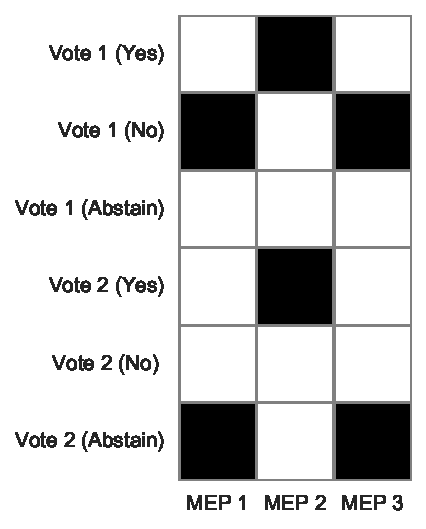
\includegraphics[width=0.38\textwidth]{figures/votematrix.pdf}
\end{center}
\vskip -1.5em
\caption{Example vote matrix: MEPs 1 and 3 voted \emph{No} on Vote 1, and abstained on Vote 2. MEP 2 Voted Yes for both.}
\label{fig:votematrix}
\end{wrapfigure}

A small example representing this encoding for two roll call votes for three different MEPs is shown in Figure \ref{fig:votematrix}.

Other potential encodings, given vote metadata and method choice are possible: a count matrix is produced by merging votes using title similarity, or policy area or committee. Detailed vote meta data is available for the 6th parliament\footnote{\url{http://personal.lse.ac.uk/hix/HixNouryRolandEPdata.htm}} from \cite{Hix821}, but is incomplete for the 7th parliament. Results are reported for vote encoding using individual votes.

MEPs who switch groups \cite{evans2012measuring} during the term present a data consistency challenge for roll call analysis using our proposed evaluation measure. MEPs who follow group voting procedure of one group for a period of the term, and then switch will be correctly clustered with the group most similar to them, but mislabelled during evaluation, as voting records remain, while group affiliation can change.

Every effort has been made to correct inconsistencies with data such as removing duplicate vote records and matching roll call records with MEP profiles to ensure MEPs represent the correct group at the time of the vote, but some inconsistencies may remain.


\begin{table}[!t]
\tablefont{
\begin{tabu} to \textwidth { X | l | r | l}
\emph{Name} & \emph{Abbreviation} & Seats & \emph{Ideology} \\ \hline
\emph{7th Term 2009--2014} &  &  & \\ \hline
European People's Party (Christian Democrats)& EPP & 274 & Conservative\\
Progressive Alliance of Socialists and Democrats& S\&D & 195 & Socialist\\
Alliance of Liberals and Democrats for Europe& ALDE & 85 & Liberal\\
European Conservatives and Reformists Group& ECR & 56 & Eurosceptic\\
Greens / European Free Alliance& G-EFA & 58 & Green\\
Group of the European United Left / Nordic Green Left& EUL-NGL & 35 & Radical Left\\
Europe of Freedom and Direct Democracy Group& EFD & 33 & Eurosceptic\\
Non-attached Members& NI & 30 & Various\\
\hline
\emph{6th Term 2004-2009} &  &  & \\ \hline
European People's Party (Christian Democrats)& EPP-ED & 288 & Conservative\\
Socialist Group in the European Parliament& PES & 217 & Socialist\\
Alliance of Liberals and Democrats for Europe& ALDE & 104 & Liberal\\
Union for Europe of the Nations Group& UEN & 40 & Nationalist\\
Greens / European Free Alliance& G/EFA & 43 & Green\\
Group of the European United Left / Nordic Green Left& EUL/NGL & 41 & Radical Left\\
Independence / Democracy Group& IND/DEM & 22 & Eurosceptic\\
Non-attached Members& NI & 30 & Various\\
\hline
\end{tabu}
}
\normalsize
\vskip 1em
\caption{Group names, seats, and ideologies for the 6th and 7th parliamentary terms. Number of seats doesn't reflect the number of MEPs active over the entire term, as some retire, or are substituted.}
\label{tbl:groups}
\end{table}


\subsection{Dimensionality Reduction}
\subsubsection {W-NOMINATE:} The \underline{W}eighted \underline{Nomina}l \underline{T}hree-step \underline{E}stimation approach \cite{wnominate} is an inductive scaling technique specifically designed for ideal point estimation of legislators using roll call data.

While the method is ubiquitous, a number of drawbacks are highlighted in \cite{clinton2003statistical}. Specifically: thresholds that exclude some votes, which results in poorer discrimination among extremist MEPs, and excluding MEPs with short voting histories. In the 7th Parliament dataset 5 of 853 MEPs and 460 of 6961 votes are excluded with the recommended settings. The methods we propose do not exclude any MEPs or Votes, and do not require setting vote or MEP specific thresholds, however they do introduce their own method specific parameters and initialisation strategies that can impact results, and do not solve the problem of parameter tuning.

\subsubsection{PCA:}
Principle Component Analysis \cite{Fodor02DRSurvey} is a commonly used linear dimension reduction technique. PCA is performed using Singular Value Decomposition on the vote data matrix. Figures \ref{fig:allmethods6} and \ref{fig:allmethods7} show the resulting visualisations.

\subsubsection{NMF:}
Given a non-negative matrix $X$, Non-negative Matrix factorization \cite{nmf1} approaches find two factor matrices $W$ and $H$ where the product of $W$ and $H$ approximates $X$. The dimensions of the factor matrices are significantly lower than the product. NMF is not commonly used for visualisation, but is a popular approach for clustering \cite{nmf} and topic modelling.

\subsubsection{t-SNE:}
t-Stochastic Neighbourhood Embedding is a popular dimensionality reduction and visualisation technique. Data is usually embedded in two or three dimensions, creating interpretable visualisations of high dimensional spaces. The stochastic nature of the process can sometimes produce visualisations that are drastically different, or contain structure that could be over-interpreted. For example, in a $2d$ plot, the $x$ and $y$ coordinates are not reliable values to use as point estimates in the same way as W-NOMINATE scores are---however, the clusters produced and relative positions of MEPs can be informative as MEPs with similar voting patterns will be clustered together. 
%Figure \ref{fig:tsne} shows projections with t-SNE applied to the vote matrix $X$.

\subsubsection{SGNS with t-SNE:}
We explore a two step process, where votes and MEPs are treated as co-occurrences---embedding votes and MEPs into a lower dimensional space with Stochastic Gradient Descent with Negative Sampling \cite{levy2014neural} and then applying t-SNE to further reduce dimensionality down to 2 or 3 for visualisation.  The two step process tends to exaggerate distances between MEPs of the same group, however this method introduces more parameters and instability, making qualitative analysis difficult and prone to over interpretation---where visualisation artefacts can be interpreted as meaningful.

\subsection{Evaluating Projections}
In order to evaluate the quality of the low dimensional projections of MEPs, we adopt Within Group Scatter and Between Group Scatter criteria, which have been widely used for the problem cluster validation \cite{desgraupes2013clustering}. Here we define our clusters as the parliamentary groups to which MEPs belong. The between group scatter quantifies differences in voting behaviour between groups, while within group scatter quantifies how cohesive a group is, or rather, how strongly party discipline dictates vote behaviour \cite{Hix821}. 

For group $k$, the within group scatter is calculated as the within group sum of squares, or $\clust{WGSS}$:
$$
\clust{WGSS} = \sum_{i\in I_{k}} ||\clust{M}_{i}-\clust{G}||^2
$$
where $G^k$ is the centroid of group $k$. The between group scatter or $BGSS$ is:
$$
BGSS=\sum_{k=1}^K n_{k}||\clust{G}-G||^2
$$
where $G^k$ is the centroid of group $k$, $G$ is the centroid of all points (representing MEPs in a $2d$ space). Small $WGSS$ values indicate tight grouping of points in a cluster, or strong party discipline in the case of MEPs and votes. Large $BGSS$ indicates large differences between groups.

%
%For each MEP $i$, the silhouette score is: %$$ %s(i) = \frac{b(i) - a(i)}{\max\{a(i),b(i)\}} %$$ where $a(i)$ is the average distance from MEP $i$ to all other MEPs in their group, and $b(i)$ is the lowest average distance to another group cluster of which the MEP is not a member of. %$s(i)$ scores close to 1 suggest that an MEP is appropriately clustered, while scores close to $-1$ suggest that the MEP would be more appropriately placed in a different, neighbouring group. The average $s(i)$ over all MEPs in a group is a measure of how tightly grouped MEPs are in the space, or rather, how strongly party discipline dictates vote behaviour\cite{Hix821}. The average $s(i)$ score across all MEPs for all groups provides a measure of quality of a method.
%
%\subsection{Dimensions in EU Votes:}
%Using the evaluation scores of projections built using different dimensions, we can try to investigate how many dimensions are optimal for each method. Figure \ref{fig:dim} shows that dimensionality reduction approaches work best for 2 or 3 dimensions in most cases. In previous work\cite{hix2006dim}, the main policy dimensions were a dominant left-right dimension, and a pro-/anti-Europe dimension. As we only use one kind of evaluation approach, there is not enough evidence to show that this 3rd dimension in the ``vote space'' is substantive.
%
\section{Results}
\label{sec:results}
We now compare the outputs generated by  W-NOMINATE and the alternative methods. Overall, in contrast to W-NOMINATE, the other methods have the advantage of significantly faster run times, but introduce method specific initialisations and parameters, which can affect visualisation output. This is most pronounced in the case of t-SNE with random initialisation, where a cluster of MEPs may be placed ``to the right'' or ``to the left'' of another group depending on the run. Initialising t-SNE with PCA produces stable arrangements of clusters in a $2d$ space, but the $x$ and $y$ values of individual MEPs are unsuitable for use as point estimates.

For $WGSS$ and $BGSS$ we exclude the non attached MEPs, as these are not members of any political group in the parliament. Ideology in the non-attached members ranges from communism, to populism, nationalism and neo-nazism.

Figure \ref{fig:wn} shows W-NOMINATE estimates that form our baseline: other approaches are compared to $WGSS$ and $BGSS$ scores derived from these results. Detailed scores by party group for the parliaments are shown in Tables \ref{tbl:6th} and \ref{tbl:7th} below. In Figure \ref{fig:wn}, the $x$ axis is interpreted as the left/right dimension, with left wing groups such as the European United Left / Nordic Green Left (EUL/NGL) placed on the left, and right wing groups such as Europe of Freedom and Democracy (IND/DEM) on the right. The $y$ axis is interpreted as capturing a pro/anti EU integration dimension, with pro-EU groups assigned estimates close to 1 and Eurosceptic or anti-EU MEPs assigned point estimates close to -1.

Figures \ref{fig:allmethods6} and \ref{fig:allmethods7} show an overview of all methods applied to the 6th and 7th parliamentary terms. In contrast to W-NOMINATE, the other methods have greater within group scatter---exaggerating differences between MEPs in the same group. While some groups are clustered more appropriately by the methods we explored, overall W-NOMINATE produces the best clustering of MEPs.

\vskip 1em

\noindent%
\begin{minipage}{\linewidth}% to keep image and caption on one page
\makebox[\linewidth]{%center image
\begin{minipage}{0.5\textwidth}
\centering
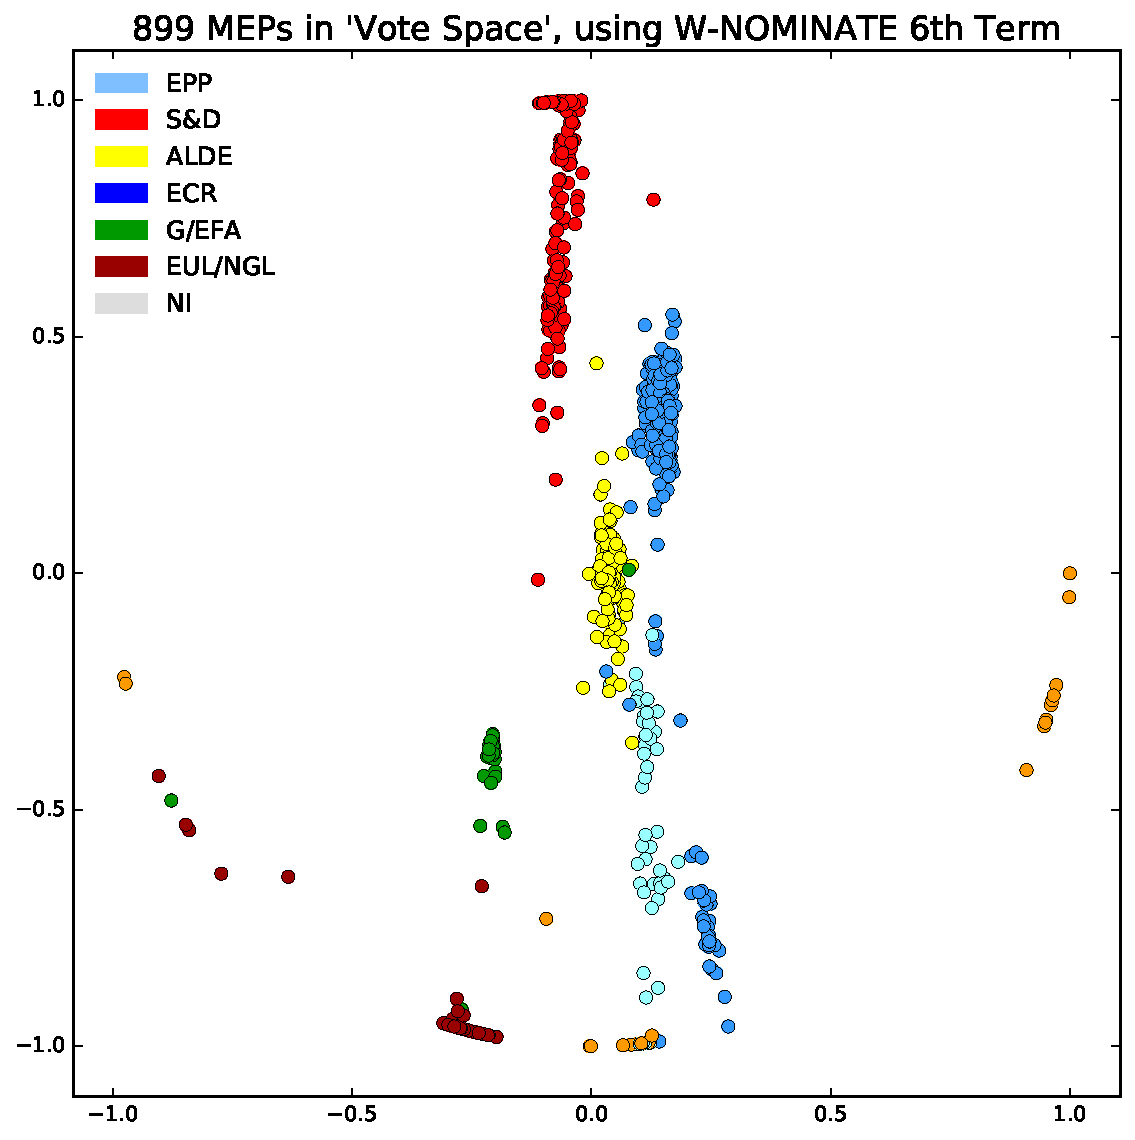
\includegraphics[width=1.0\textwidth]{figures/W-NOMINATE-6th.pdf}
\end{minipage}%
\begin{minipage}{0.5\textwidth}
\centering
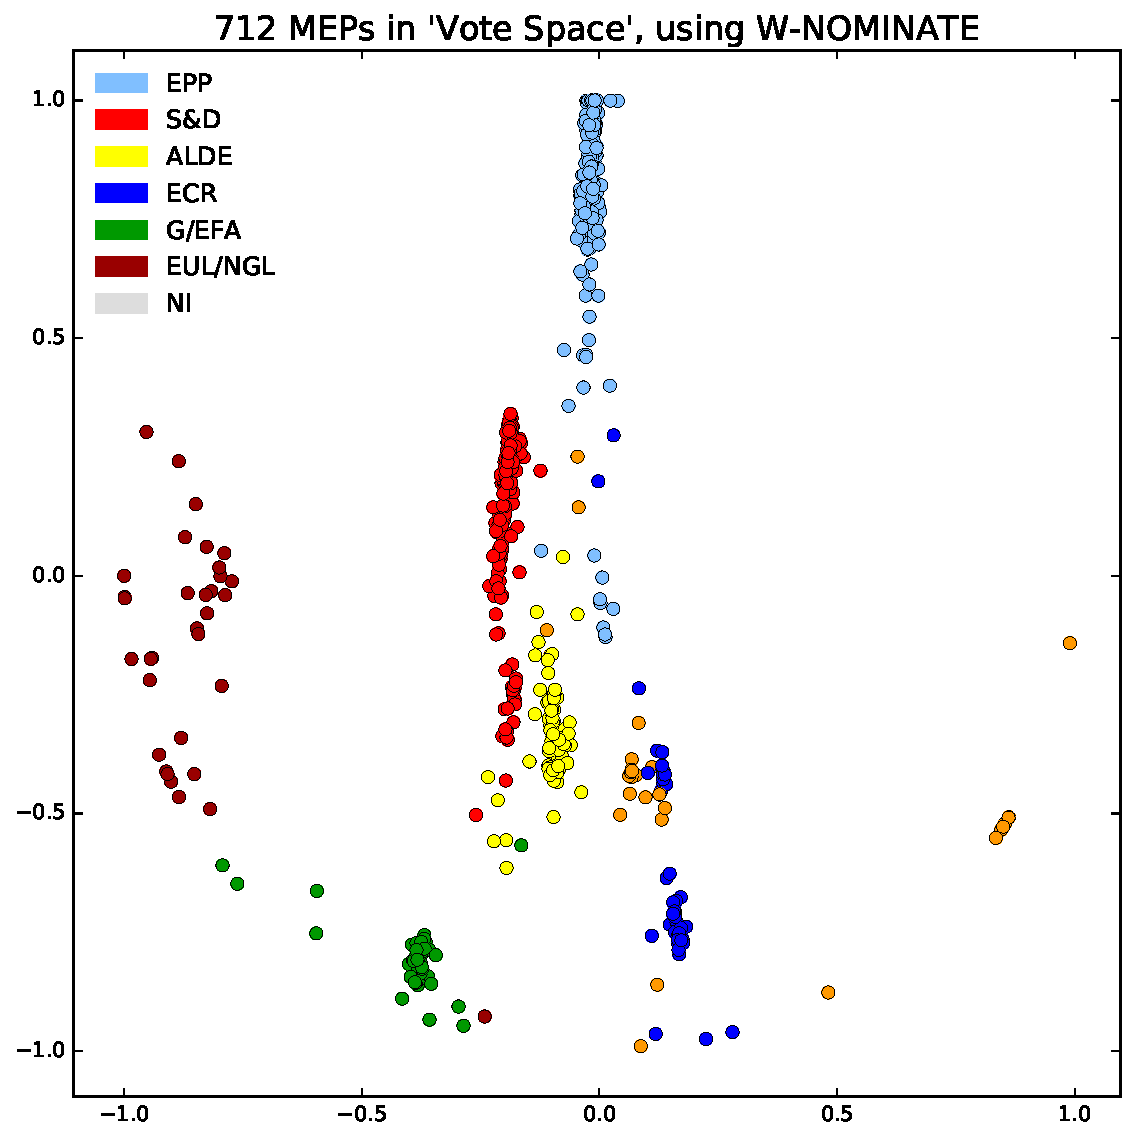
\includegraphics[width=1.0\textwidth]{figures/W-NOMINATE-7th.pdf}
\end{minipage}}
\captionof{figure}{W-NOMINATE scales for the 6th (left) and 7th (right) Parliaments.}\label{fig:wn}
\end{minipage}

%\begin{figure}[!h]
%    \centering
%    \begin{minipage}{0.5\textwidth}
%        \centering
%        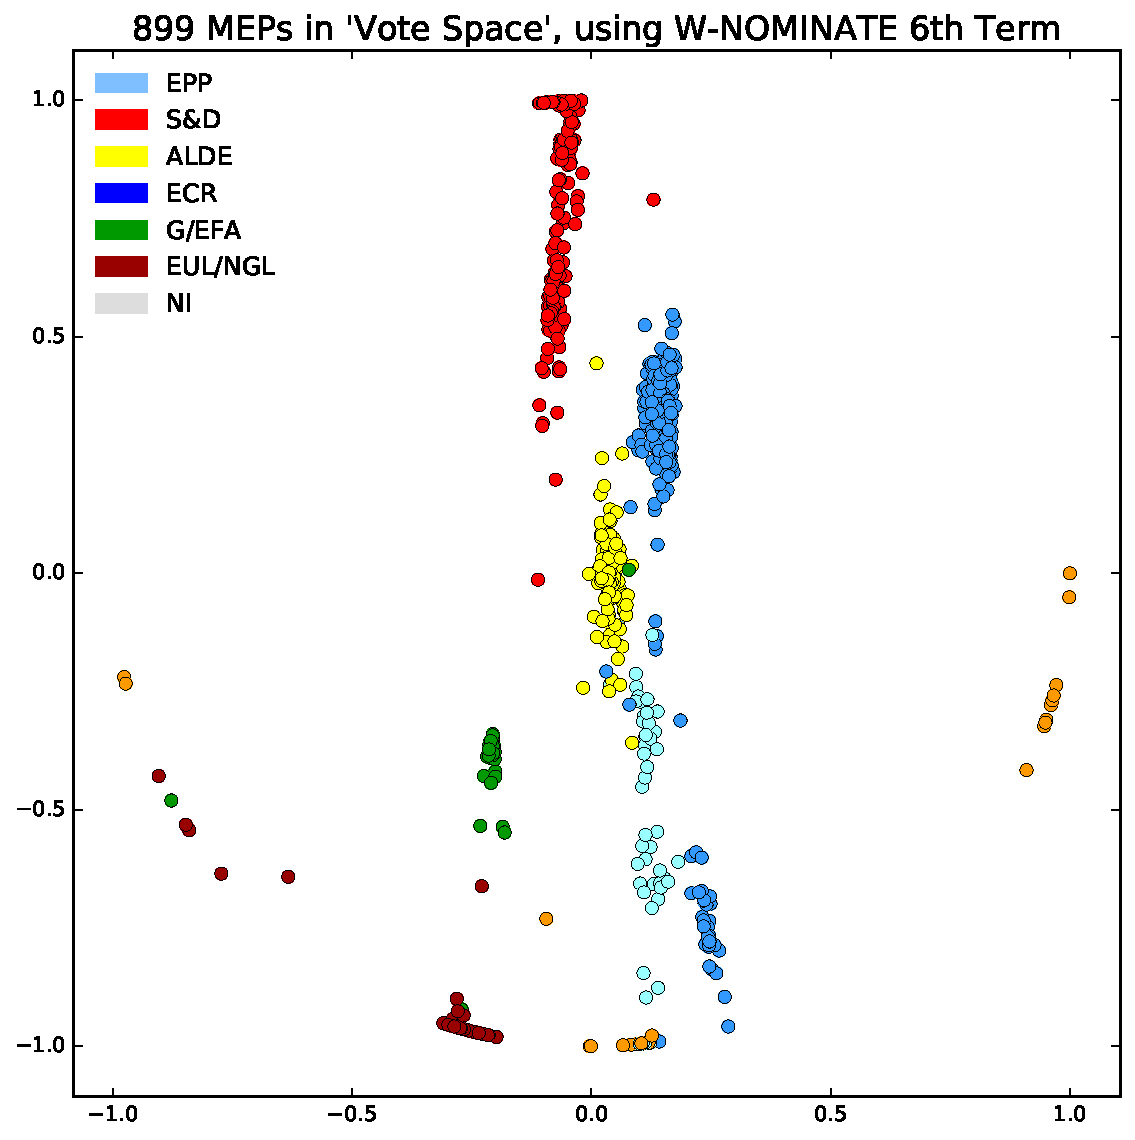
\includegraphics[width=1.0\textwidth]{figures/W-NOMINATE-6th.pdf}
%        %\caption{6th}
%        %\label{fig:dim6}
%    \end{minipage}%
%    \begin{minipage}{0.5\textwidth}
%        \centering
%        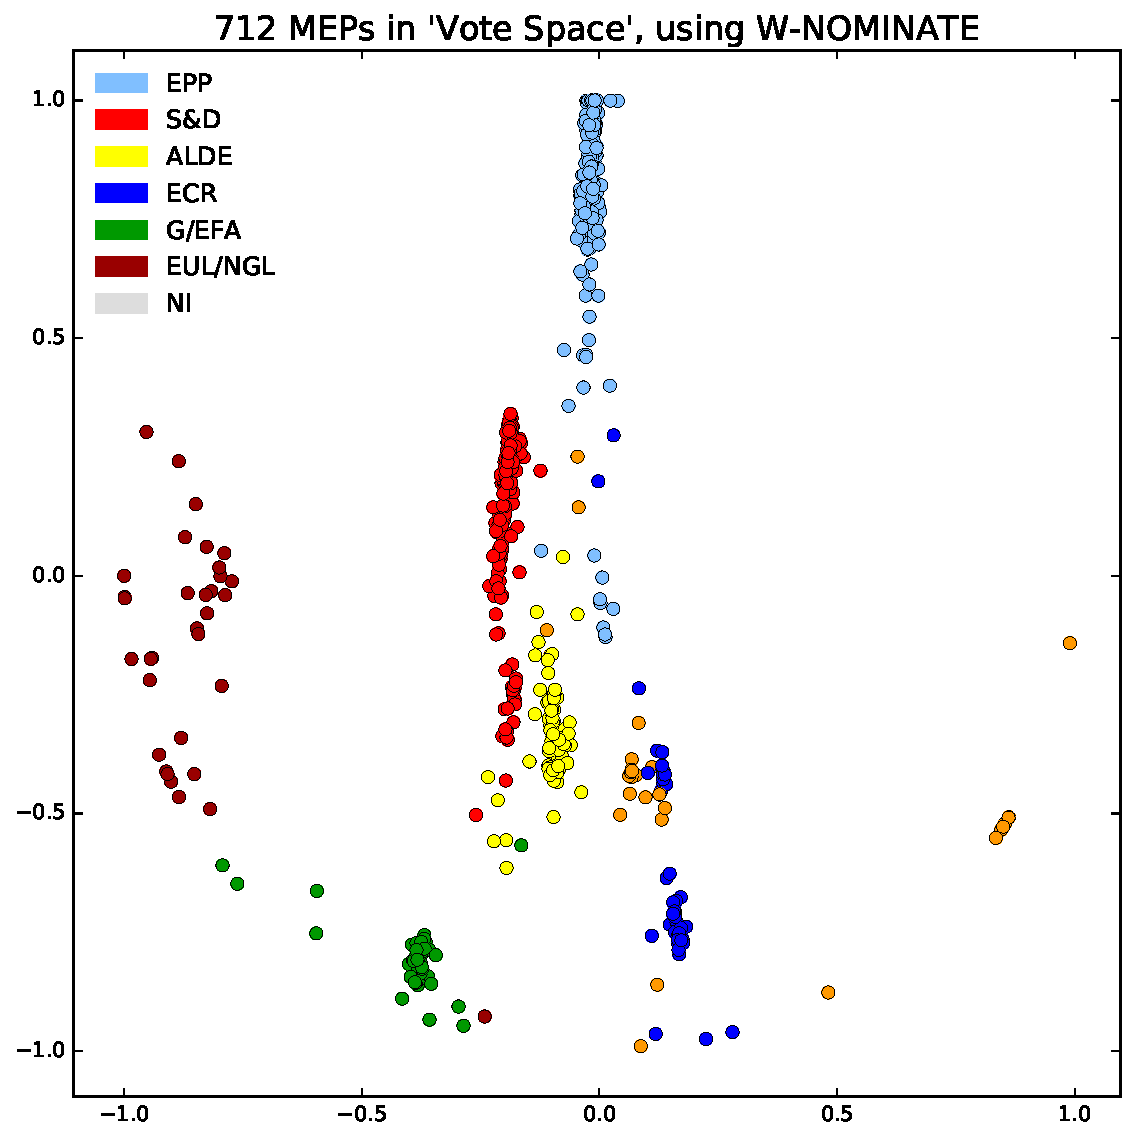
\includegraphics[width=1.0\textwidth]{figures/W-NOMINATE-7th.pdf}
%        %\caption{7th}
%        %\label{fig:dim7}
%    \end{minipage}
%    \caption{W-NOMINATE scales for the 6th (left) and 7th (right) Parliaments.}\label{fig:wn}
%\end{figure}


\subsection{6th Term}

The 6th term began in 2004, and ended in 2009. In total there are records for 899 MEPs. MEPs sometimes join the parliament at different times, retire, or are replaced. We include an MEP in a group if they have a record of a vote in the dataset.

%\begin{figure}[!h]
%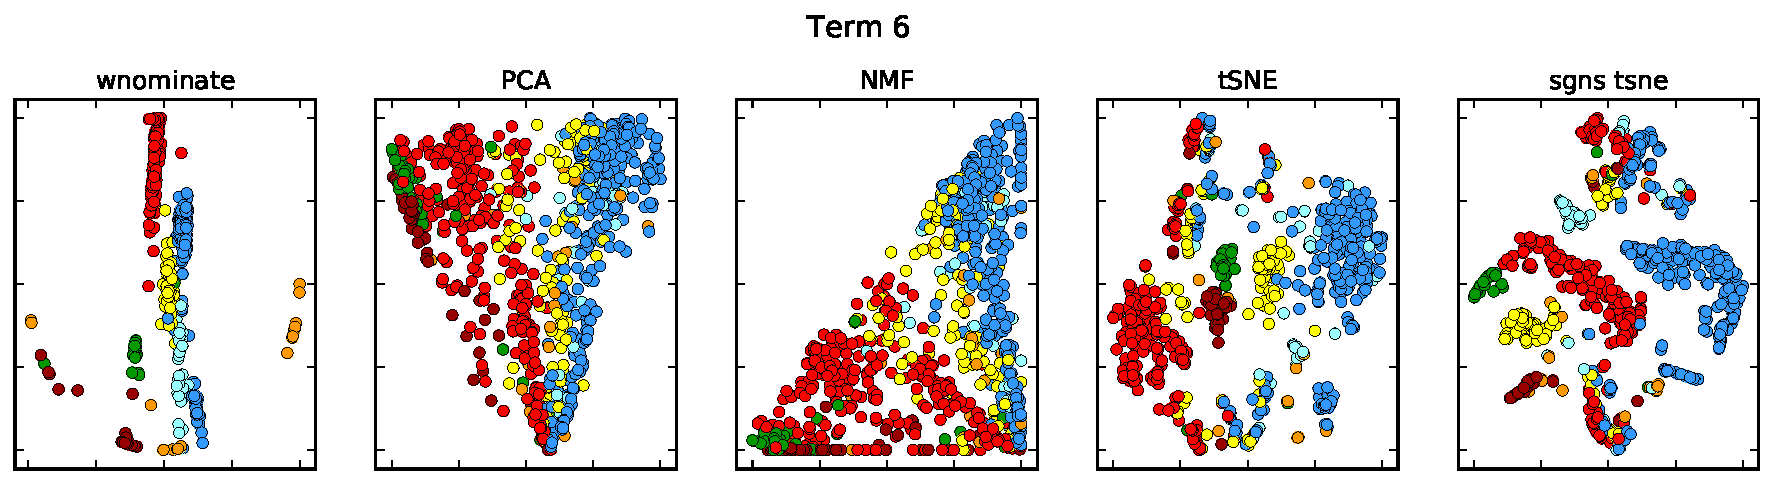
\includegraphics[width=\textwidth]{figures/term6.pdf}
%\caption{Overview of visualisations built on 6th Term voting records. Points are in clusters coloured by group.}
%\label{fig:allmethods6}
%\end{figure}

%\vskip 1em

\noindent%
\begin{minipage}{\linewidth}% to keep image and caption on one page
\makebox[\linewidth]{%center image
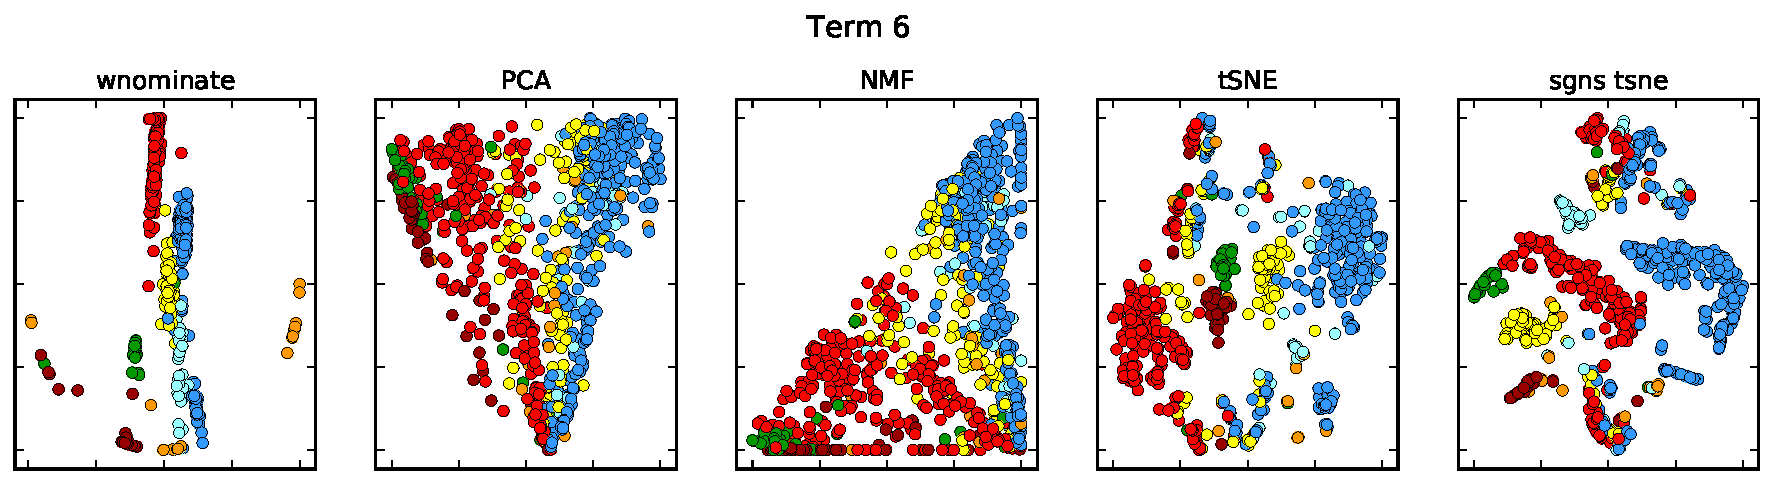
\includegraphics[width=\textwidth,keepaspectratio=true]{figures/term6.pdf}}
\captionof{figure}{Overview of visualisations built on 6th Term voting records. Points are in clusters coloured by group.}\label{fig:allmethods6}
\end{minipage}

%\noindent%
%\begin{minipage}{\linewidth}% to keep image and caption on one page
%\makebox[\linewidth]{%center image
%%%%%%%%%%%%
%\captionof{figure}{.}\label{}
%\end{minipage}

%\vskip -2em

\begin{table}[!h]
\small
\begin{tabu} to \textwidth {X[m,l] X[m,r] X[m,r] X[m,r] X[m,r] X[m,r] X[m,r]}
\toprule
    Group &  MEPs &  WNOM. &  PCA &  NMF &  t-SNE &  SGNS \\
\midrule
   EPP-ED &   340 &      43.22 &    139.52 &    108.88 &     144.38 &     101.81 \\
      PES &   264 &      11.14 &    104.53 &     79.22 &      74.27 &      85.12 \\
     ALDE &   125 &       1.22 &     50.96 &     39.07 &      32.10 &      40.65 \\
      UEN &    51 &       3.32 &     16.66 &     13.73 &      16.51 &      12.67 \\
  EUL/NGL &    48 &       2.17 &     16.24 &     14.39 &       5.79 &      11.70 \\
    G/EFA &    44 &       1.08 &     10.47 &      9.52 &       2.54 &       5.71 \\
  IND/DEM &    27 &      13.68 &      9.79 &      9.14 &      12.63 &       8.28 \\ \hline
    Overall &   899 &      75.84 &    348.18 &    273.95 &     288.23 &     265.93 \\
\bottomrule
\end{tabu}
\vskip 1em
\caption{$WGSS$: Within Group Scatter, votes from 6th Term. Smaller values indicate that MEPs in a group are close to other group members in the vote space.}
\label{tbl:6th}
\end{table}

\vskip -2em

\begin{table}[!h]
\begin{tabu} to \textwidth {X[m,l] X[m,r] X[m,r] X[m,r] X[m,r] X[m,r] X[m,r]}
\toprule
    Group &  MEPs &  WNOM. &  PCA &  NMF &  t-SNE &  SGNS \\
\midrule
   EPP-ED &   340 &       4.88 &     64.84 &    124.63 &      84.77 &      71.64 \\
      PES &   264 &     106.88 &     45.62 &     88.63 &     104.96 &       6.75 \\
     ALDE &   125 &       6.48 &      3.19 &      4.61 &       1.32 &      16.06 \\
      UEN &    51 &      30.13 &      5.45 &     10.42 &       5.13 &       7.37 \\
  EUL/NGL &    48 &      67.56 &     28.44 &     49.66 &       4.32 &      24.17 \\
    G/EFA &    44 &      19.27 &     34.64 &     62.29 &       1.76 &      32.62 \\
  IND/DEM &    27 &      18.92 &      3.35 &      2.08 &       4.57 &       5.10 \\ \hline
    Overall &   899 &     254.13 &    185.53 &    342.32 &     206.84 &     163.71 \\
\bottomrule
\end{tabu}
\vskip 1em
\caption{$BGSS$: Between Group Scatter, using votes from the 6th Term. Larger values indicate greater separation between clusters of MEPs.}
\end{table}


\subsection{7th Term}

The 7th parliament was elected in 2009 and finished in 2014. Between the 7th and the 6th parliaments there were a number of changes made to groups, including new members and affiliation switches with existing MEPs.

%\vskip -2em
%\begin{figure}[!h]
%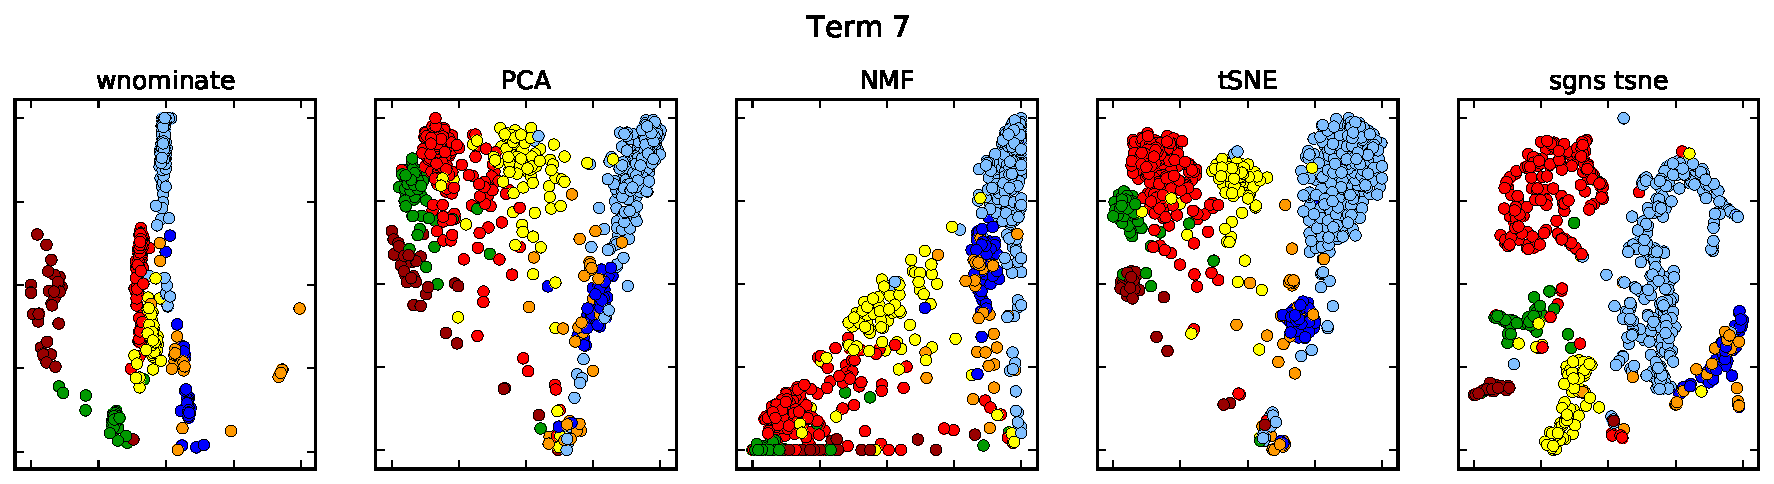
\includegraphics[width=\textwidth]{figures/term7.pdf}
%\caption{Overview of visualisations built on 7th Term voting records. Points are in clusters coloured by group.}
%\label{fig:allmethods7}
%\end{figure}

\vskip 1em

\noindent%
\begin{minipage}{\linewidth}% to keep image and caption on one page
\makebox[\linewidth]{%center image
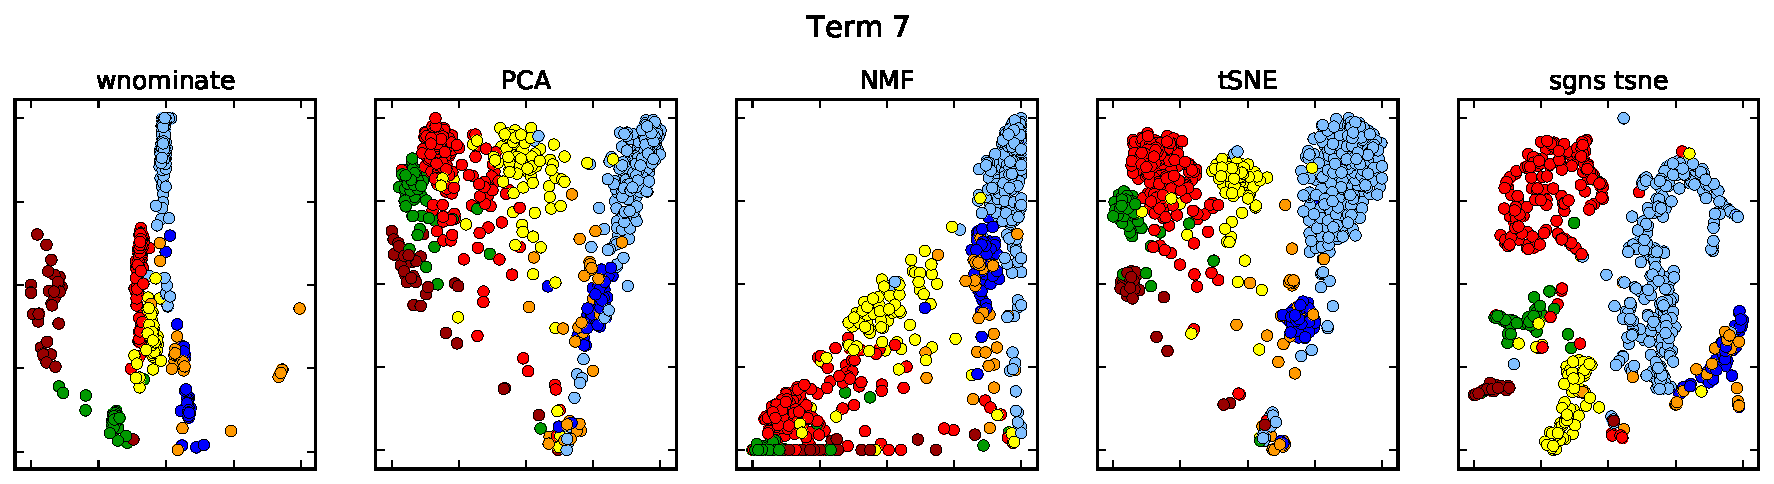
\includegraphics[width=\textwidth,keepaspectratio=true]{figures/term7.pdf}}
\captionof{figure}{Overview of visualisations built on 7th Term voting records. Points are in clusters coloured by group.}\label{fig:allmethods7}
\end{minipage}

%\vskip -2em

\begin{table}[!h]
\begin{tabu} to \textwidth {X[m,l] X[m,r] X[m,r] X[m,r] X[m,r] X[m,r] X[m,r]}
\toprule
    Group &  MEPs &  WNOM. &  PCA &  NMF &  t-SNE &  SGNS \\
\midrule
      EPP &   267 &      12.18 &     41.54 &     36.81 &      49.82 &      68.47 \\
      S\&D &   184 &       6.72 &     26.75 &     23.88 &      27.21 &      32.23 \\
     ALDE &    85 &       0.96 &     15.55 &     13.91 &      12.36 &      14.33 \\
    G/EFA &    56 &       0.70 &      7.89 &      7.06 &       6.88 &       2.99 \\
      ECR &    54 &       3.17 &      3.80 &      2.83 &       2.97 &       3.20 \\
  EUL/NGL &    35 &       2.59 &      6.45 &      5.96 &       5.31 &       4.60 \\
      EFD &    31 &       5.85 &      6.97 &      3.91 &       6.50 &       4.22 \\ \hline
    Overall &   712 &      32.17 &    108.95 &     94.35 &     111.06 &     130.03 \\
\bottomrule
\end{tabu}
\vskip 1em
\caption{$WGSS$: Within Group Scatter, votes from 7th Term. Smaller values indicate that MEPs in a group are close to other group members in the vote space.}
\label{tbl:7th}
\end{table}

\vskip -2em

\begin{table}[!h]
\begin{tabu} to \textwidth {X[m,l] X[m,r] X[m,r] X[m,r] X[m,r] X[m,r] X[m,r]}
\toprule
    Group &  MEPs &  WNOM. &  PCA &  NMF &  t-SNE &  SGNS \\
\midrule
      EPP &   267 &     125.35 &    132.34 &    281.77 &     121.42 &      44.48 \\
      S\&D &   184 &       1.45 &     86.05 &    187.74 &      76.81 &      81.13 \\
     ALDE &    85 &      22.32 &      2.64 &      4.05 &       2.11 &      40.16 \\
    G/EFA &    56 &      57.96 &     44.33 &     92.59 &      42.30 &      25.37 \\
     ECR &    54 &      39.57 &     28.56 &     18.36 &      29.45 &      44.77 \\
  EUL/NGL &    35 &      23.11 &     35.09 &     43.00 &      31.59 &      37.77 \\
      EFD &    31 &      16.52 &     20.80 &      7.84 &      20.19 &      25.22 \\ \hline
   Overall &   712 &     286.29 &    349.81 &    635.33 &     323.86 &     298.89 \\
\bottomrule
\end{tabu}
\vskip 1em
\caption{$BGSS$: Between Group Scatter, using votes from the 7th Term. Larger values indicate greater separation between clusters of MEPs.}
\end{table}

%\begin{figure}[!h]
%    \centering
%    \begin{minipage}{0.5\textwidth}
%        \centering
%        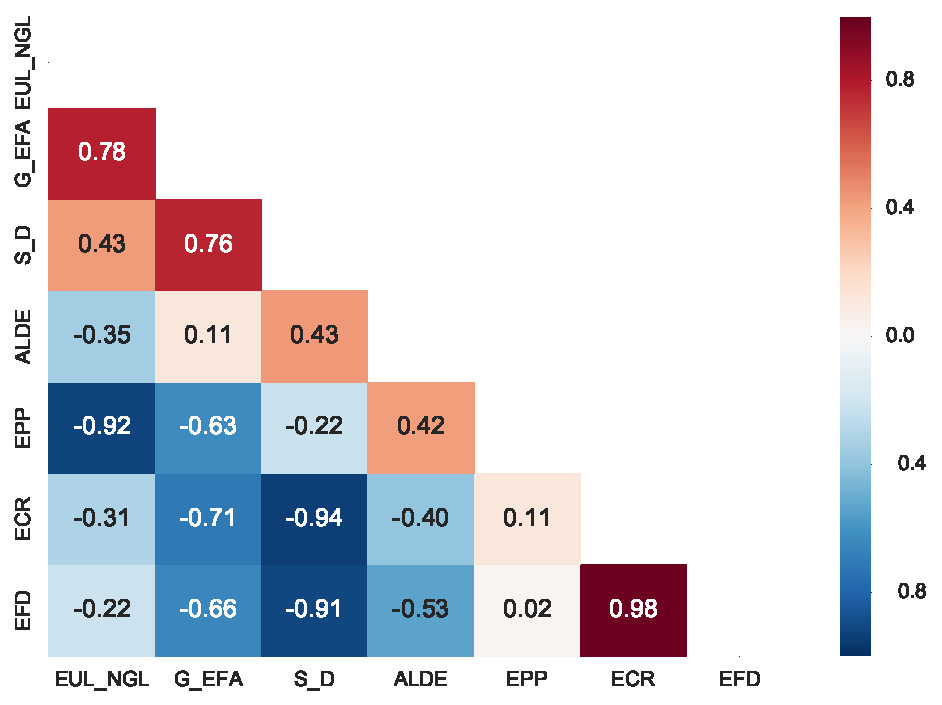
\includegraphics[width=1.0\textwidth]{figures/term7survey.pdf}
%        %\caption{6th}
%        %\label{fig:dim6}
%    \end{minipage}%
%    \begin{minipage}{0.5\textwidth}
%        \centering
%        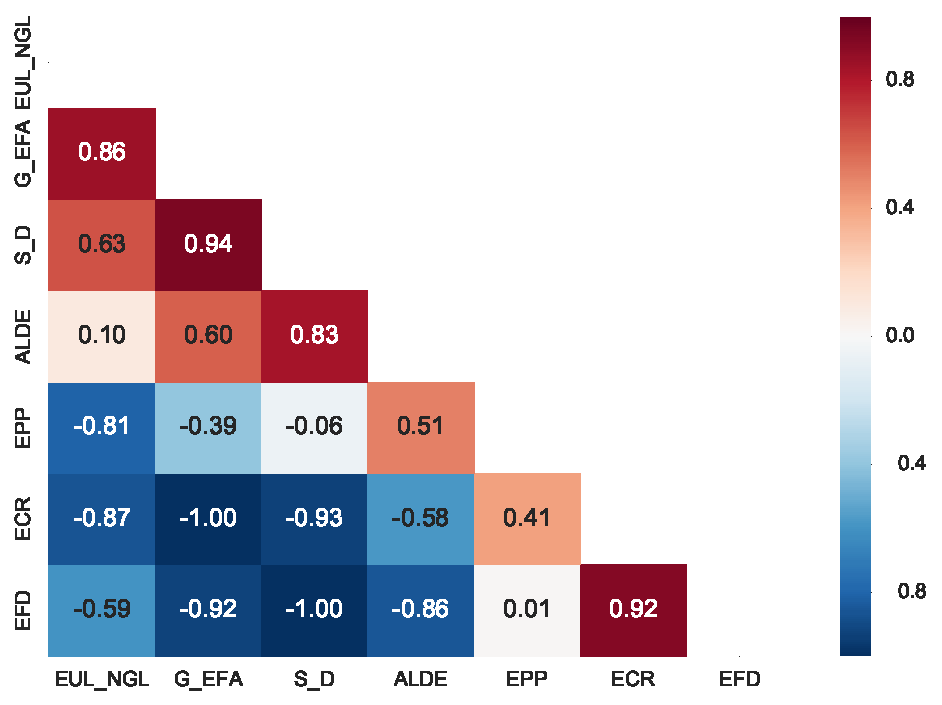
\includegraphics[width=1.0\textwidth]{figures/term7survey_tsne.pdf}
%        %\caption{7th}
%        %\label{fig:dim7}
%    \end{minipage}
%    \caption{Pairwise Similarity of groups using expert surveys, and pairwise similarity using cluster centroids}\label{fig:survey}
%\end{figure}

\section{Discussion}
While the methods we explore do not out perform the well established and widely used W-NOMINATE approach using a cluster validation based evaluation, there are a number of useful recommendations we can make when using different methods: NNDSVD initialization strategy for NMF produces most stable results; PCA initialization for t-SNE can help with stability of results. Even so, there is still a risk of over interpreting the structure that t-SNE produces. Before drawing any conclusions from visualisations made with t-SNE, we recommend paying particular attention to the implementation and parameters, especially the learning rate used during optimization. The SGNS approach allows most flexibility with encoding votes, but is the least stable method. The dimensions themselves from NMF, or t-SNE are not as useful for point estimates compared to W-NOMINATE, but the relative positions of cluster centroids offer a useful measure of similarity between groups.

Many techniques are applicable if we treat roll call vote scaling as a dimensionality reduction problem. All methods that aim to project or embed high dimensional data in a low dimensional space introduce some uncertainty and instability. Uncertainty in point estimates can come from many sources: from data quality issues and encoding schemes, to parameter and initialization choices, to visualisation choices. Given these issues, one advantage that the alternative methods we explored have is their speed and efficiency: multiple runs under different settings can highlight errors in ideal point estimates more clearly.

In terms of evaluation, expert surveys \cite{mcelroy2012policy} or coded party manifestos \cite{manifesto} may offer better benchmarks for differences between groups and MEPs. Producing annotations and expert surveys is a costly task however, and there are currently no expert judgements or annotations available for all votes for a full term.

\section{Conclusion}
We applied several commonly used dimensionality reduction techniques to voting records in the EU parliament. While all techniques tend to exaggerate distances between MEPs of the same group, they can perhaps be useful for quantifying within-party differences, or treating cluster centroids as points---similarities between groups.

Applying similar methods to speeches and using point estimates derived from our proposed methods as alternatives in downstream tasks is ongoing, as well as comparisons of other projection techniques, applied to more recent data covering the current 8th parliamentary term.

% --- ACKNOWLEDGE FUNDING SOURCES
\vspace{3mm}
\noindent\textbf{Acknowledgement:} This publication has emanated from research conducted with the support of Science Foundation Ireland (SFI) under Grant Number SFI/12/RC/2289.

% --- BIBLIOGRAPHY
\bibliographystyle{splncs03}
\bibliography{aics-votes} 

\end{document}
